%%%%%%%%%%%%%%%%%%%%%%%%%%%%%%%%%%%%%%%%%
% Beamer Presentation
% LaTeX Template
% Version 1.0 (10/11/12)
%
% This template has been downloaded from:
% http://www.LaTeXTemplates.com
%
% License:
% CC BY-NC-SA 3.0 (http://creativecommons.org/licenses/by-nc-sa/3.0/)
%
%%%%%%%%%%%%%%%%%%%%%%%%%%%%%%%%%%%%%%%%%

%----------------------------------------------------------------------------------------
%	PACKAGES AND THEMES
%----------------------------------------------------------------------------------------

\documentclass{beamer}

\mode<presentation> {

% The Beamer class comes with a number of default slide themes
% which change the colors and layouts of slides. Below this is a list
% of all the themes, uncomment each in turn to see what they look like.

%\usetheme{default}
%\usetheme{AnnArbor}
%\usetheme{Antibes}
%\usetheme{Bergen}
%\usetheme{Berkeley}
%\usetheme{Berlin}
%\usetheme{Boadilla}
%\usetheme{CambridgeUS}
%\usetheme{Copenhagen}
%\usetheme{Darmstadt}
%\usetheme{Dresden}
%\usetheme{Frankfurt}
%\usetheme{Goettingen}
%\usetheme{Hannover}
%\usetheme{Ilmenau}
%\usetheme{JuanLesPins}
%\usetheme{Luebeck}
%\usetheme{Madrid}
%\usetheme{Malmoe}
%\usetheme{Marburg}
%\usetheme{Montpellier}
%\usetheme{PaloAlto}
%\usetheme{Pittsburgh}
%\usetheme{Rochester}
%\usetheme{Singapore}
\usetheme{Szeged}
%\usetheme{Warsaw}

% As well as themes, the Beamer class has a number of color themes
% for any slide theme. Uncomment each of these in turn to see how it
% changes the colors of your current slide theme.

%\usecolortheme{albatross}
%\usecolortheme{beaver}
%\usecolortheme{beetle}
%\usecolortheme{crane}
%\usecolortheme{dolphin}
%\usecolortheme{dove}
%\usecolortheme{fly}
%\usecolortheme{lily}
%\usecolortheme{orchid}
%\usecolortheme{rose}
%\usecolortheme{seagull}
%\usecolortheme{seahorse}
%\usecolortheme{whale}
%\usecolortheme{wolverine}

%\setbeamertemplate{footline} % To remove the footer line in all slides uncomment this line
%\setbeamertemplate{footline}[page number] % To replace the footer line in all slides with a simple slide count uncomment this line

%\setbeamertemplate{navigation symbols}{} % To remove the navigation symbols from the bottom of all slides uncomment this line
}

\usepackage{graphicx} % Allows including images
\usepackage{booktabs} % Allows the use of \toprule, \midrule and \bottomrule in tables
\usepackage{array}
\usepackage{color}
\usepackage{url}
\usepackage[T2A]{fontenc}
\usepackage[utf8]{inputenc} 
\usepackage[export]{adjustbox}
\usepackage{amsmath}
\usepackage{sidecap}
\usepackage{mathtools}
%\usepackage[english,serbian]{babel}
\usepackage[english,serbianc]{babel} %ukljuciti babel sa ovim opcijama, umesto gornjim, ukoliko se koristi cirilica

%----------------------------------------------------------------------------------------
%	TITLE PAGE
%----------------------------------------------------------------------------------------

\title[Семинарски МСНР]{Примена техника машинског учења у статичкој верификацији софтвера}
\author{	Лазар Ранковић ????/2016 \\
		Немања Мићовић ????/2016 \\
		Урош Стегић 447/2016
}
\institute[МАТФ]{Математички факултет}
\date{\today}

\begin{document}

\begin{frame}
\titlepage
\end{frame}

\begin{frame}
\frametitle{Садржај}
\tableofcontents
\end{frame}

%----------------------------------------------------------------------------------------
%	PREZENTACIJA
%----------------------------------------------------------------------------------------



%-----------------------------------------------------------------
\section{Статичка верификација}

\begin{frame}
\frametitle{Мотивација}
\begin{itemize}
	\item Нуклеарна експлозија
	\item Трећи светски рат
	\item Не производе се више јафолитанке
\end{itemize}
\end{frame}
%-----------------------------------------------------------------
\begin{frame}
\frametitle{Методи верификације}
\begin{itemize}
	\item Апстрактна интерпретација
 	\item Проверавање ограничених модела
 	\item Симболичко израчунавање
\end{itemize}
\end{frame}
%-----------------------------------------------------------------



%-----------------------------------------------------------------
\section{Машинско учење}

\begin{frame}
\frametitle{Мотивација}
\begin{itemize}
 	\item Алгоритамски нерешиви проблеми
	\item Предикција
\end{itemize}
\end{frame}
%-----------------------------------------------------------------
\begin{frame}
\frametitle{Регресија}
\begin{figure}
\centering
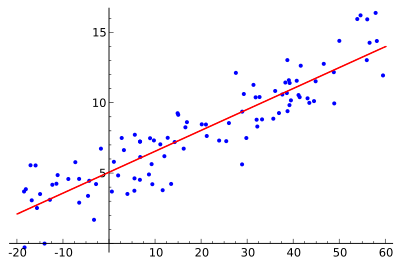
\includegraphics[scale=0.4]{slike/linearna_regresija.png}
\end{figure}
\end{frame}
%-----------------------------------------------------------------
\begin{frame}
\frametitle{Класификација}
\begin{itemize}
 	\item Препознавање објеката на фотографији
 	\item Разврставање непожељне поште
 	\item Класификација стања програма
\end{itemize}
\end{frame}
%-----------------------------------------------------------------
\begin{frame}
\frametitle{Стабло одлучивања}
\begin{figure}
\centering
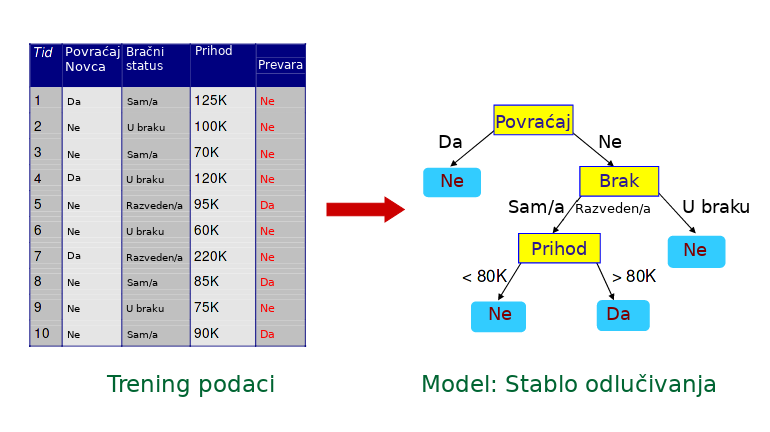
\includegraphics[scale=0.4]{slike/decision_tree.png}
\end{figure}
\end{frame}
%-----------------------------------------------------------------
\begin{frame}
\frametitle{Метода подржавајућих вектора}
\begin{figure}
\centering
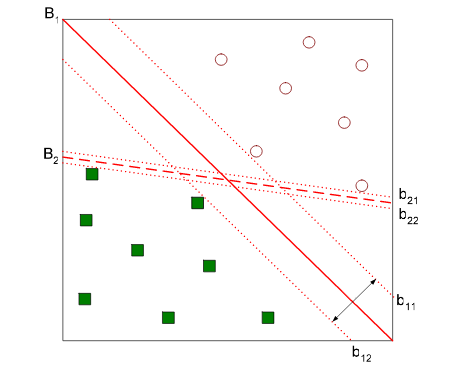
\includegraphics[scale=0.4]{slike/svm.png}
\end{figure}
\end{frame}
%-----------------------------------------------------------------



%-----------------------------------------------------------------
\section{Примене МУ у статичкој верификацији}

\begin{frame}
\frametitle{Неки наслов}
\begin{itemize}
\item Неки метод 1
\item Неки метод 2
\end{itemize}
\end{frame}
%-----------------------------------------------------------------
\begin{frame}
\Huge{\centerline{Хвала на пажњи}}
\end{frame}
%-----------------------------------------------------------------



%-----------------------------------------------------------------
\end{document} 